\documentclass[letter,10pt,twocolumn,openany]{dndbook}

% Use babel or polyglossia to automatically redefine macros for terms
% Armor Class, Level, etc...
% Default output is in English; captions are located in lib/dndstring-captions.sty.
% If no captions exist for a language, English will be used.
%1. To load a language with babel:
%	\usepackage[<lang>]{babel}
%2. To load a language with polyglossia:
%	\usepackage{polyglossia}
%	\setdefaultlanguage{<lang>}
\usepackage[english]{babel}
% For further options (multilanguage documents, hypenations, language environments...)
% please refer to babel/polyglossia's documentation.

\usepackage[utf8]{inputenc}
\usepackage[singlelinecheck=false]{caption}
\usepackage{lipsum}
\usepackage{listings}
\usepackage{shortvrb}
\usepackage{stfloats}
\usepackage{hyperref}

\captionsetup[table]{labelformat=empty,font={sf,sc,bf,},skip=0pt}

\MakeShortVerb{|}

\lstset{%
  basicstyle=\ttfamily,
  language=[LaTeX]{TeX},
  breaklines=true,
}

\title{Lilli Nackle’s Index of the Arcane}
\author{Jens Keim\\(aka pepper-jk)}
\date{\today}

\begin{document}

\frontmatter

\maketitle

\tableofcontents

\mainmatter

\chapter{Magic Items}

\DndItemHeader{Dagger of Disinterest}{Weapon (dagger), unknown rarity (requires attunement)}
You gain a +2 bonus to attack and damage rolls made with this magic weapon.\\

This magic weapon has 3 charges. When you hit an enemy with this weapon, you can choose to expend one of its charges to heal you or an allied creature within 60 feet by half the damage done by your attack rounded down plus the creatures constitution modifier.\\
The dagger regains 1d3 expended charges daily at dawn. If you healed yourself with its abilities on the day before, half the result of the recharge dice and round down.\\

%DM only
%\subparagraph{Curse} This dagger is cursed. If you heal yourself, your maximum hit points reduce by the amount of hit points you healed yourself with the dagger this day after your next long rest (after you regained your hit points from your rest). If you are reduced to 0 hit points by this, you crumble to ash and are contained in the dagger. You can be freed and resurrectted with the remove curse spell.\\
%This curse can not be detected by the identify spell until the caster saw someone die this way and is looking for the cause of it.

\begin{figure}
    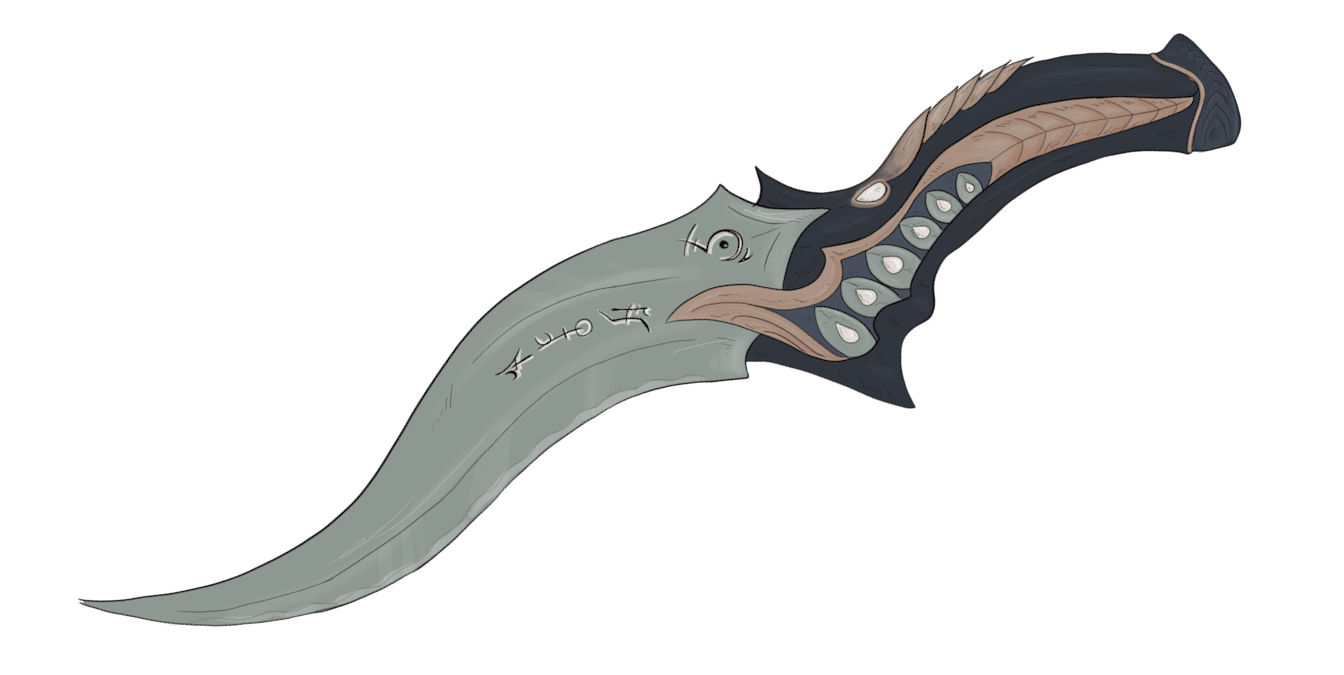
\includegraphics[width=9cm]{images/dagger_of_disinterest.png}
    \caption{Dagger of Disinterest}
\end{figure}

\DndItemHeader{Druid Totem}{Wonderous item, unknown rarity (requires attunement by a druid)}

This magic item is a small locket made of wood, that takes the shape of an animal of the owners choice.
Though most druids change it to the animal they wild shape to.\\

It can be used as a spell casting focus.\\

Once attuned to the totem, you can use an action to embed a gem into it.
The totem can house up to three gems at a time.
An embedded gem is considered attuned.
Once a gem is embedded into the totem it can only be removed again during a long rest.\\

Each gem comes with a number of charges.
During your wild shape, you can expend charges to activate one of the gems effects.
If the effect allows you to cast a spell, you expend spell slots as you would normally.
The totem regains 1d3 expended charges daily at dawn.
Those charges are mutually assigned to a random Gem, that can regain charges.

\pagebreak

\DndItemHeader{Water Gem}{3 charges total}

\subparagraph{Life Transfer}
The first time you hit with an attack during an action, you may expend a charge to mark each creature you hit during this action.
The next attack that hits a marked creature deals 2d8 necrotic damage.
The attacker gains hit points equal to that damage.

\subparagraph{The Essence of Life}
When you touch a wounded creature that is not an undead or construct, you can expend a charge.
If you do so, you can either cast \textit{Cure Wounds} or \textit{Healing Word} with range touch.

\subparagraph{At Home in Water}
As a bonus action, you may expend a charge to gain a swimming speed equal to your walking speed until the end of your next turn.

\DndItemHeader{Air Gem}{Common, 3 charges total}

\subparagraph{Swift Step}
As a bonus action, you can expend one charge to double your movement speed until the end of your next turn.
Alternatively you may expend all three charges to double your movement for 1 minute.

\subparagraph{Feathered Jump}
Your body becomes extremely light.
You can expend a charge to cast \textit{Jump} on yourself, as a bonus action.

\subparagraph{Winged Beast}
You sprout astral wings from your back.
As a bonus action, you may expend a charge to gain a flying speed equal to your walking speed until the end of your next turn.

\DndItemHeader{Earth Gem}{Rare, 6 charges total}

\subparagraph{Stone Born}
As a bonus action, you may expend three charges and cast \textit{Stoneskin} on yourself.

\subparagraph{Rock Shield}
You reach out and cover your ally with a rocky shield sprouting from one of your extremities.
As a reaction to an ally getting hit by an attack within your reach, you can expend two charges to intercept the attack and take half of the damage yourself.

\DndItemHeader{Leaf Gem}{Common, 3 charges total}

\subparagraph{Entangling Sprouts}
Vines sprout from the wounds you inflict and entangle the creatures.
The first time you hit with an attack during an action, you can expend a charge.
If you do so, each target you hit during this action is entangled by vines and is restrained until the end of their next turn.

\subparagraph{Spike Growth}
As a bonus action, you may expend two charges and cast \textit{Spike Growth}.

\DndItemHeader{Psionic Gem}{Very rare, 3 charges total}
% spell casting focus?

\subparagraph{Psionics}
You can detect, identify and recognize psionic based magic, including illusions and magical disguises.

\subparagraph{Psionic Penetration}
When you cast a spell, you can expend 1 charge to ignore magic resistance of psionic casters.

\subparagraph{Telepathy}
During your wild shape you can communicate telepathically with any willing creature within 30 feet of you.
Additionally, you can form a telepathic link with a willing creature.
While the two are linked, you can communicate telepathically with the other creature as long as you are within 1 mile of each other.

\begin{figure}
    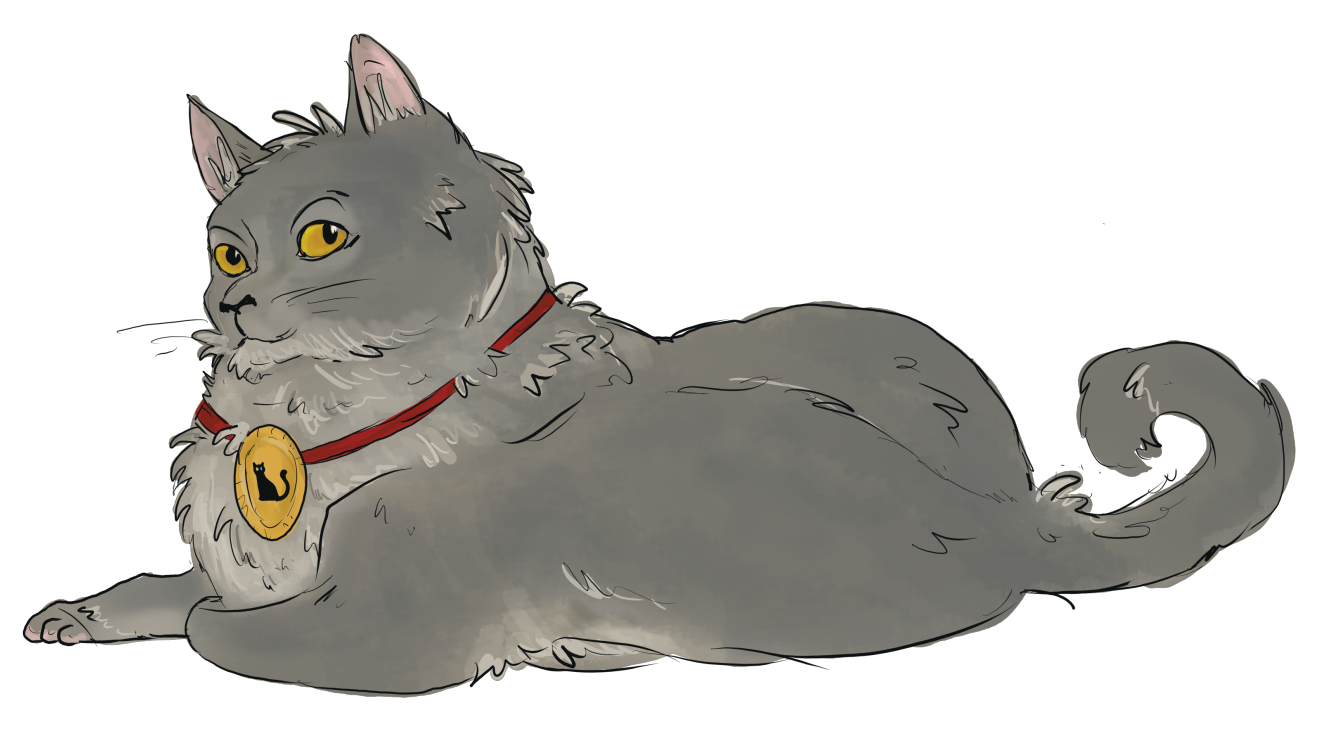
\includegraphics[width=9cm]{images/cat.png}
    \caption{A cat wearing the druid totem. She is not a druid, she just likes the locket.}
\end{figure}

\begin{figure}
    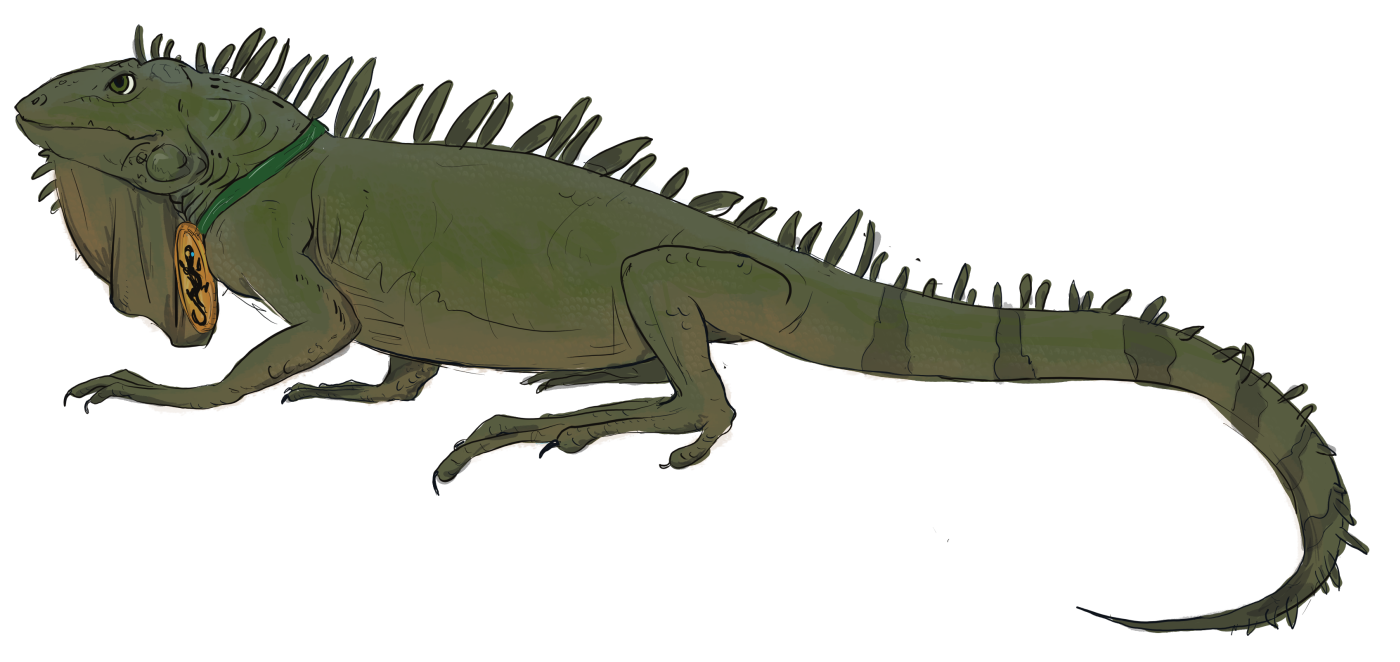
\includegraphics[width=9cm]{images/iguana.png}
    \caption{A druid in his natural habitat sunning himself, while wearing the druid totem.}
\end{figure}

\begin{figure}
    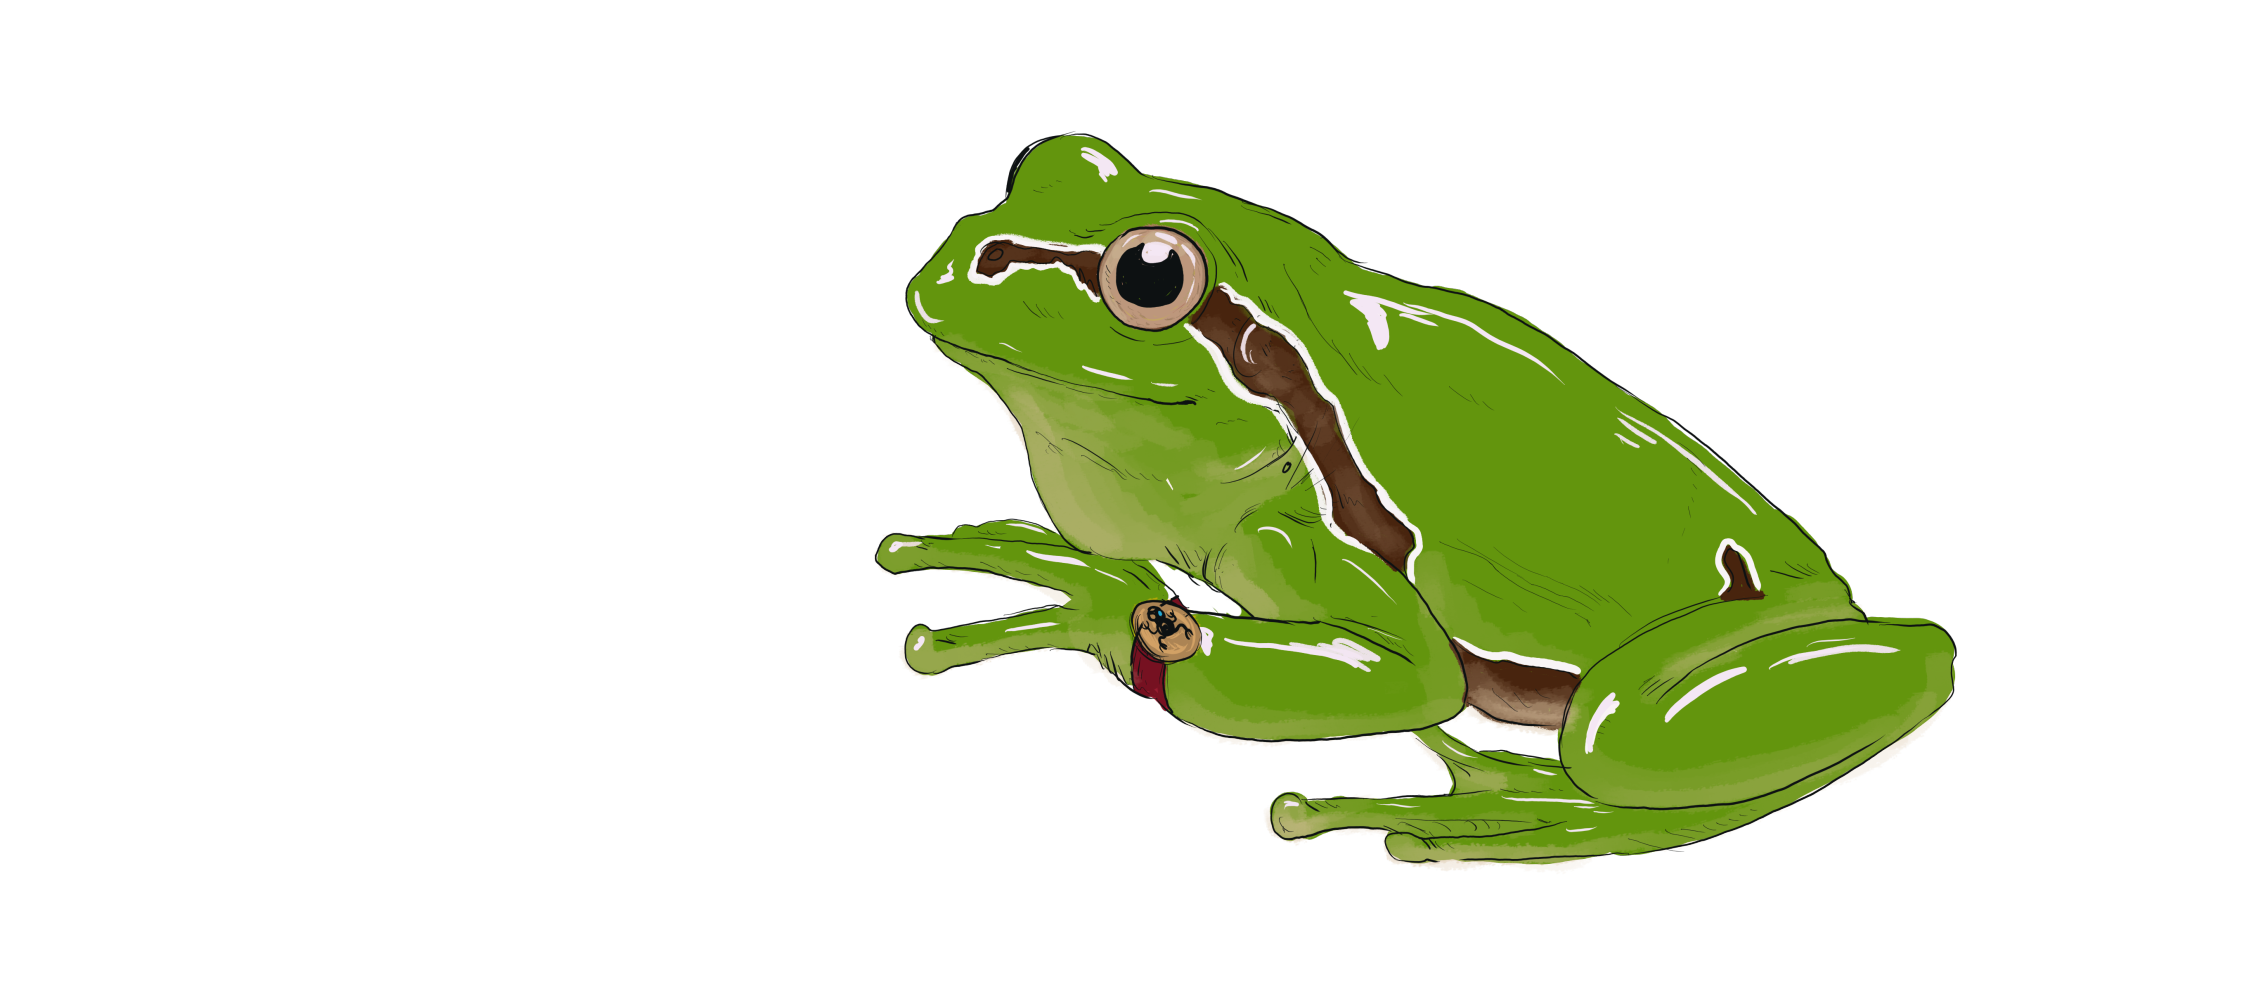
\includegraphics[width=9cm]{images/frog.png}
    \caption{A druid wild shaped into a frog wearing the druid totem.}
\end{figure}

\pagebreak

\DndItemHeader{Fey Scroll}{Scroll, unknown rarity (requires attunement by a warlock)}

A fey scroll works just like a spell scroll. In addition if you can attune to it, you can merge it with your book of shadows. The scroll is then mended into the book. This consumes the scroll, meaning it is no longer an item on its own.\\
Non-ritual spells are known to the books owner, once they were added to the book in this way and only this way.\\
If the scroll merged into your book of shadows in this way, contains an eldritch invocation the owner of the book gains that invocation in addition to the invocations he already knows. Invocations gained this way can not be replaced, when the owner of the book gains a level.

\begin{figure}
    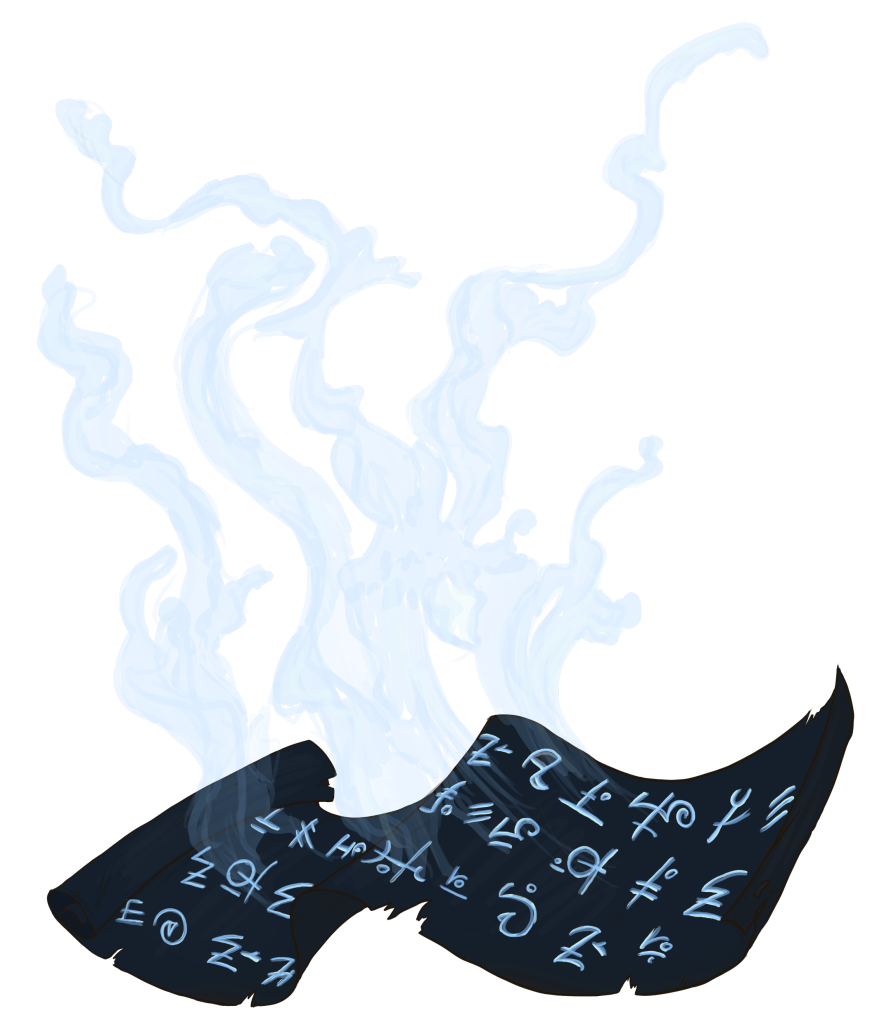
\includegraphics[width=9cm]{images/fey_scroll.png}
    \caption{Fey Scroll}
\end{figure}

\DndItemHeader{Manual of Maneuvers, Volume X}{Wondrous item, unknown rarity (requires a battle master)}
This book describes maneuver exercises, and its words are charged with magic.
If you spend 24 hours over a period of 6 days or fewer studying the book's contents and practicing its guidelines, you gain a maneuver.
The maneuver is determined by which Volume of the manuals you have, see the Manual of Maneuvers Volumes table \ref{table_maneuvers}.
The manual then loses its magic, but regains it in ten years.\\

\begin{figure}
    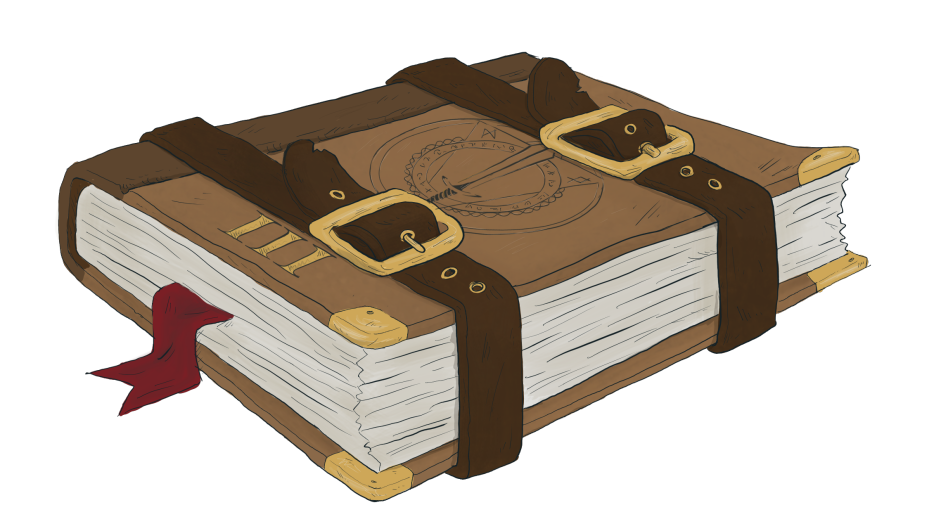
\includegraphics[width=9cm]{images/manual_of_maneuvers.png}
    \caption{Manual of Meneuvers}
\end{figure}

\begin{table}
    \centering
    \begin{dndtable}[XX]
        \textbf{Volume} & \textbf{Maneuver} \\
        3 & Fearless Rescue \\
        4 & Move Forward \\
        7 & Battle Inspiration
    \end{dndtable}
    \caption{Manual of Maneuvers Volumes}
    \label{table_maneuvers}
\end{table}

% \pagebreak

\DndItemHeader{Ring of Horeos}{Ring, legendary (requires attunement)}

These magic rings were crafted by the Lunar priests of Selûne over a century ago.
They were distributed to the most honorable among the knights of Selûne and Valor Guardians.
It is unknown to most how many were created and most of them were lost during the Siege of Murann.
The rings that remain lie dormant until a worthy heir appears before them, who carries a love for Murann in their heart.

\paragraph{Sentience}
A \textit{ring of heroes} is a sentient neutral good item with an Intelligence of 12, a Wisdom of 10, and a Charisma of 12.
It has hearing and normal vision out to a range of 60 feet.
The ring communicates by transmitting emotions, sending a tingling sensation through the wielder's hand when it wants to communicate something it has sensed.
It can communicate more explicitly, through visions or dreams, when the wielder is either in a trance or asleep.

\paragraph{Personality}
Every \textit{ring of heroes} seeks to protect Murann at all costs.
It is reluctant to leave the city.
It likes everything moon related and is faithful to Selûne.
When fighting evil shapechangers, specifically lycanthropes, it enjoys itself.
Otherwise the personality resembles the one of its previous wielder(s).

\paragraph{Dormant}
A \textit{ring of heroes} grants the following benefits in its dormant state:
\begin{itemize}
    \item A \textit{ring of heroes} acts as a \textit{Ring of Spell Storing}.
    \item During a long rest you can choose 5 levels worth of spells from the moon spell list to fill the rings slots.
    % TODO: what is the spell casting modifier?
\end{itemize}

\paragraph{Awakened}
Once a \textit{ring of heroes} reaches an awakened state, it gains the following properties:

\begin{itemize}
    \item \textbf{Perceive True Shape}
    You can perceives the original form of a shapechanger or a creature that is transformed by magic within 60ft.
    You gain Darkvision out to 60 feet, as long as it is not new moon.
    During a full moon you gain Truesight out to 60 feet.
    If you already have either Darkvision or Truesight, your range increases by 60 feet instead.
    \item \textbf{Turn Lycanthropes}
    Once per day as an action, you present the ring and it shines a bright moon light.
    Each lycanthrope that can see within 30 feet of you must make a Wisdom saving throw.
    If the creature fails its saving throw, it is turned for 1 minute or until it takes any damage.

    A turned creature must spend its turns trying to move as far away from you as it can, and it can't willingly move to a space within 30 feet of you. It also can't take reactions. For its action, it can use only the Dash action or try to escape from an effect that prevents it from moving. If there's nowhere to move, the creature can use the Dodge action.
\end{itemize}

% FIXME: additional slots? maybe split slots (2 awakened, 3 exalted) (1 awakened, 1 exalted)

\paragraph{Exalted}
Once a \textit{ring of heroes} reaches an exalted state, it gains the following properties:

\begin{itemize}
    \item The ring stores an additional five slots worth of spells that can only be used by the moon spell list.
    \item \textbf{Temporal Salvation}
    If you die while wearing this ring, you vanish and reappear in an unoccupied space within 5 feet of the space you left (or the nearest unoccupied space).
    You have a number of hit points equal to 3d6 + your Constitution modifier.
    If your hit point maximum is lower than the number of hit points you regain, your hit point maximum rises to a similar amount.
    If you have any levels of exhaustion, reduce your level of exhaustion by 1.
    Once this feature is used, it can not be used again until the next full moon.
    \item \textbf{Moon Chosen}
    If you wear this ring you ignore the lineage (race) requirement, when attuning to a \textit{Moonblade}.
    (You do not need to be attuned to the ring to benefit from this.
    But the ring needs to be in its exalted state.)
\end{itemize}

\begin{table}
    \centering
    \begin{dndtable}[XX]
        \textbf{Level} & \textbf{Spells} \\
        1 & faerie fire \\
        2 & calm emotions, moonbeam \\
        3 & moon blade \\
        5 & moon path \\
    \end{dndtable}
    \caption{Moon spell list}
    \label{table_moon_spells}
\end{table}

\DndItemHeader{Ring of Rings}{Ring, uncommon}

This magic ring takes the physical place of up to ten rings.
If any of those rings are magical, they retain any effects from being worn or attuned.
While you wear this ring, the other rings are stored in a pocket dimension.
If you take the ring of, your rings magically reappear on the finger you last wore them on.

The ring looks like a mundane ring made of silver (worth 20 gp).
However, you can also use a bonus action to speak the ring's command word and cause the ring to assume the appearance of any of your rings.

\DndItemHeader{Ring of the Dork}{Ring, uncommon}

When wearing this magical ring, you appear to be wearing up to ten rings of an appearance of your choice.
Although illusions, these rings withstand a physical inspection as long as they are on your fingers.
However, if you take a ring off, it disappears.
If you take the ring off, any other ring created by it disappears and ring assumes the form of a mundane ring made of gold (worth 50 gp).

If you create a ring that bears status, for example a sigel ring of a family other then your own, the creature inspecting the ring makes a Wisdom (Insight) check against your Charisma (Deception) check.
On a success, they notice that the ring is a fake just as they would with a badly forged ring.

\DndItemHeader{Rings of Sending}{Ring, uncommon}

Rings of sending come in pairs.
While you wear one ring, you can use an action to cast the sending spell from it.
The target is the bearer of the other ring.
If no creature bears the other ring, you know that fact as soon as you use the ring and don't cast the spell.

Once sending is cast through the rings, they can't be used again until the next dawn.
If one of the rings in a pair is destroyed, the other one becomes nonmagical.

\begin{DndComment}{Wedding Rings of Sending Variant}
    When used in the a wedding ceremony, crafted or bought for a spouse,
    the Rings of Sending gains an additional number of casting of the sending spell equal to the started decades of the couples relationship.
\end{DndComment}

\DndItemHeader{Zinlee's Amulet of Commoner Protection}{Wondrous item, uncommon}
Wearing this item raises the maximum HP of the wearer to 25
If the wearer has more then 25 maximum HP it has no effect.

\begin{figure}
    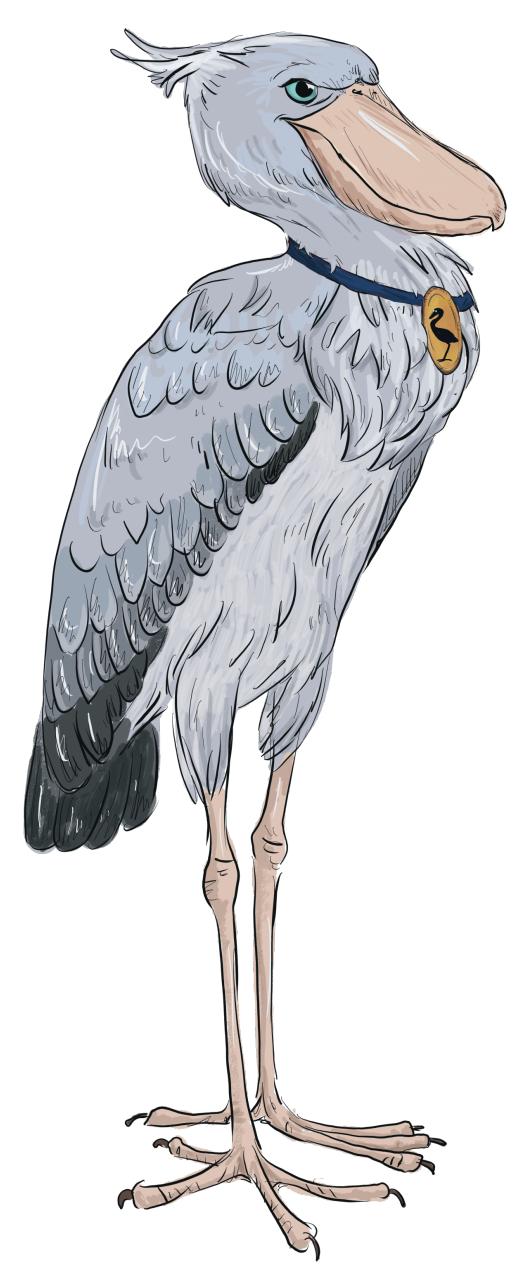
\includegraphics[width=6.5cm]{images/shoebill.png}
    \caption{A druid wearing the druid totem, while wild shaped into a shoebill.}
\end{figure}

\chapter{Spells}

% Fey Hex works like the normal hex spell, but gives disadvantage on attack rolls or saving throws (your choice) [instead of ability checks] until the end of your next turn.

\DndSpellHeader
  {Fey Hex}
  {3rd-level enchantment}
  {1 bonus action}
  {90 feet}
  {V, S, M (the petrified eye of a pixie)}
  {Concentration, up to 1 minute}

You place a curse on a creature that you can see within range. Until the spell ends you deal an extra 1d6 necrotic damage to the target whenever you hit it with an attack. The target has disadvantage on attack rolls or saving throws (your choice) until the end of your next turn.\\
If the target drops to 0 hit points before this spell ends. you can use a bonus action on a subsequent turn of yours to curse a new creature.\\
A remove curse cast on the target ends this spell early.\\
At Higher Levels. When you cast this spell using a spell slot of 5th level, you can maintain your concentration on the spell for up to 1 hour.

\chapter{Character Options}

\section{Eldritch Invocation}

\DndItemHeader{Bouncing Blast}{Prerequisite: eldritch blast cantrip}

When you hit a creature with eldritch blast, once per short rest you can spread the damage onto the creatures around it.

Any creature you deem friendly is not affected, every other creature within 15 feet of the target takes half damage.

\section{Maneuvers}

\subparagraph{Battle Inspiration}
When either you or a friendly creature you can see within 30 feet of you makes an attack roll, you can expend a superiority die to roll the die and add half the result to that attack roll. You can do this before or after the attack roll is made, but before you know whether or not it was a hit. If choosing another creature, you must use your reaction to use this maneuver, and the creature must be able to either see or hear you to benefit.

\subparagraph{Fearless Rescue}
»One of your allies falls, and without regard for your own wellbeing, you rush to make the attacker pay. Your bravery inspires your ally to fight on.«\\
Once per short rest when an enemy within 30 feet of you reduces an ally below 10 hit points, you can as a Reaction expend a superiority die to move to the nearest square from which you can attack that enemy and attack that enemy. You add the superiority die to the attack's damage roll.
The ally then regains 1d6 hit points and 1d6 hit points more for every opportunity attack you provoke while moving to the target.

\subparagraph{Move Forward}
When you hit a creature with a weapon attack, you may expend a superiority die to move your party forward.
As a reaction one of your allies may use the dash action.
You also add the superiority die to the attack's damage roll.

\chapter{Special Features}

\subsection{Power of a Water Guardian}

Once per day, you can use a short rest to meditate as the guardian showed you. You make a Wisdom Check. If the result is 10 or higher you can use the \textbf{Frost Jab} Action once until the end of your next long rest. If the result is 15 or higher you instead can use the \textbf{Frost Kick} Action instead.

\paragraph{Frost Jab} Melee Weapon Attack str/dex to hit, reach 5ft., one target. Hit: 1d8+str/dex bludgeoning damage plus 3d6 cold damage.

\paragraph{Frost Kick} Melee Weapon Attack str/dex to hit, reach 5ft., one target. Hit: 2d6+str/dex bludgeoning damage plus 4d6 cold damage. If the target is a creature, it must succeed a Strength saving throw or be knocked prone, the DC of which is the result of your attack roll or 15, whatever is the lowest.

\backmatter

\chapter{Licensing}

The magic items, spells and invocations are to be considered \textbf{open game content}, but feel free to credit me.

Any flavor text and art is licensed under \href{https://creativecommons.org/licenses/by-sa/4.0/legalcode}{\textit{Creative Commons Attribution Share Alike 4.0 International}} (\textbf{CC-BY-SA-4.0}).

\section{Credit}

\paragraph{Art} Zilpep (\href{https://www.deviantart.com/zilpep}{\textbf{deviantart.com/Zilpep}})
\paragraph{Writing} Jens Keim (aka pepper-jk)

\section{Open Game License}

OPEN GAME LICENSE Version 1.0a The following text is the property of Wizards of the Coast, LLC. and is Copyright 2000 Wizards of the Coast, Inc (“Wizards”). All Rights Reserved.

1. Definitions: (a)”Contributors” means the copyright and/or trademark owners who have contributed Open Game Content; (b)”Derivative Material” means copyrighted material including derivative works and translations (including into other computer languages), potation, modification, correction, addition, extension, upgrade, improvement, compilation, abridgment or other form in which an existing work may be recast, transformed or adapted; (c) “Distribute” means to reproduce, License, rent, lease, sell, broadcast, publicly display, transmit or otherwise distribute; (d)”Open Game Content” means the game mechanic and includes the methods, procedures, processes and routines to the extent such content does not embody the Product Identity and is an enhancement over the prior art and any additional content clearly identified as Open Game Content by the Contributor, and means any work covered by this License, including translations and derivative works under copyright law, but specifically excludes Product Identity. (e) “Product Identity” means product and product line names, logos and identifying marks including trade dress; artifacts; creatures characters; stories, storylines, plots, thematic elements, dialogue, incidents, language, artwork, symbols, designs, depictions, likenesses, formats, poses, concepts, themes and graphic, photographic and other visual or audio representations; names and descriptions of characters, Spells, enchantments, personalities, teams, personas, likenesses and Special abilities; places, locations, environments, creatures, Equipment, magical or supernatural Abilities or Effects, logos, symbols, or graphic designs; and any other trademark or registered trademark clearly identified as Product identity by the owner of the Product Identity, and which specifically excludes the OPEN Game Content; (f) “Trademark” means the logos, names, mark, sign, motto, designs that are used by a Contributor to Identify itself or its products or the associated products contributed to the Open Game License by the Contributor (g) “Use”, “Used” or “Using” means to use, Distribute, copy, edit, format, modify, translate and otherwise create Derivative Material of Open Game Content. (h) “You” or “Your” means the licensee in terms of this agreement.

2. The License: This License applies to any Open Game Content that contains a notice indicating that the Open Game Content may only be Used under and in terms of this License. You must affix such a notice to any Open Game Content that you Use. No terms may be added to or subtracted from this License except as described by the License itself. No other terms or Conditions may be applied to any Open Game Content distributed using this License.

3. Offer and Acceptance: By Using the Open Game Content You indicate Your acceptance of the terms of this License.

4. Grant and Consideration: In consideration for agreeing to use this License, the Contributors grant You a perpetual, worldwide, royalty-free, nonexclusive License with the exact terms of this License to Use, the Open Game Content.

5. Representation of Authority to Contribute: If You are contributing original material as Open Game Content, You represent that Your Contributions are Your original Creation and/or You have sufficient rights to grant the rights conveyed by this License.

6. Notice of License Copyright: You must update the COPYRIGHT NOTICE portion of this License to include the exact text of the COPYRIGHT NOTICE of any Open Game Content You are copying, modifying or distributing, and You must add the title, the copyright date, and the copyright holder’s name to the COPYRIGHT NOTICE of any original Open Game Content you Distribute.

7. Use of Product Identity: You agree not to Use any Product Identity, including as an indication as to compatibility, except as expressly licensed in another, independent Agreement with the owner of each element of that Product Identity. You agree not to indicate compatibility or co-adaptability with any Trademark or Registered Trademark in conjunction with a work containing Open Game Content except as expressly licensed in another, independent Agreement with the owner of such Trademark or Registered Trademark. The use of any Product Identity in Open Game Content does not constitute a Challenge to the ownership of that Product Identity. The owner of any Product Identity used in Open Game Content shall retain all rights, title and interest in and to that Product Identity.

8. Identification: If you distribute Open Game Content You must clearly indicate which portions of the work that you are distributing are Open Game Content.

9. Updating the License: Wizards or its designated Agents may publish updated versions of this License. You may use any authorized version of this License to copy, modify and distribute any Open Game Content originally distributed under any version of this License.

10. Copy of this License: You MUST include a copy of this License with every copy of the Open Game Content You Distribute.

11. Use of Contributor Credits: You may not market or advertise the Open Game Content using the name of any Contributor unless You have written permission from the Contributor to do so.

12. Inability to Comply: If it is impossible for You to comply with any of the terms of this License with respect to some or all of the Open Game Content due to statute, judicial order, or governmental regulation then You may not Use any Open Game Material so affected.

13. Termination: This License will terminate automatically if You fail to comply with all terms herein and fail to cure such breach within 30 days of becoming aware of the breach. All sublicenses shall survive the termination of this License.

14. Reformation: If any provision of this License is held to be unenforceable, such provision shall be reformed only to the extent necessary to make it enforceable.

15. COPYRIGHT NOTICE

    Open Game License v 1.0a Copyright 2000, Wizards of the Coast, LLC.System Reference Document 5.1 Copyright 2016, Wizards of the Coast, LLC.; Authors Mike Mearls, Jeremy Crawford, Chris Perkins, Rodney Thompson, Peter Lee, James Wyatt, Robert J. Schwalb, Bruce R. Cordell, Chris Sims, and Steve Townshend, based on original material by E. Gary Gygax and Dave Arneson.

    Lilli Nackle’s Index of the Arcane Copyright 2019-2021, Jens Keim

END OF LICENSE

\end{document}
